\documentclass[man]{apa6}
\usepackage{lmodern}
\usepackage{amssymb,amsmath}
\usepackage{ifxetex,ifluatex}
\usepackage{fixltx2e} % provides \textsubscript
\ifnum 0\ifxetex 1\fi\ifluatex 1\fi=0 % if pdftex
  \usepackage[T1]{fontenc}
  \usepackage[utf8]{inputenc}
\else % if luatex or xelatex
  \ifxetex
    \usepackage{mathspec}
  \else
    \usepackage{fontspec}
  \fi
  \defaultfontfeatures{Ligatures=TeX,Scale=MatchLowercase}
\fi
% use upquote if available, for straight quotes in verbatim environments
\IfFileExists{upquote.sty}{\usepackage{upquote}}{}
% use microtype if available
\IfFileExists{microtype.sty}{%
\usepackage{microtype}
\UseMicrotypeSet[protrusion]{basicmath} % disable protrusion for tt fonts
}{}
\usepackage{hyperref}
\hypersetup{unicode=true,
            pdftitle={How do children produce negation?},
            pdfauthor={First Author~\& Ernst-August Doelle},
            pdfkeywords={keywords},
            pdfborder={0 0 0},
            breaklinks=true}
\urlstyle{same}  % don't use monospace font for urls
\usepackage{graphicx,grffile}
\makeatletter
\def\maxwidth{\ifdim\Gin@nat@width>\linewidth\linewidth\else\Gin@nat@width\fi}
\def\maxheight{\ifdim\Gin@nat@height>\textheight\textheight\else\Gin@nat@height\fi}
\makeatother
% Scale images if necessary, so that they will not overflow the page
% margins by default, and it is still possible to overwrite the defaults
% using explicit options in \includegraphics[width, height, ...]{}
\setkeys{Gin}{width=\maxwidth,height=\maxheight,keepaspectratio}
\IfFileExists{parskip.sty}{%
\usepackage{parskip}
}{% else
\setlength{\parindent}{0pt}
\setlength{\parskip}{6pt plus 2pt minus 1pt}
}
\setlength{\emergencystretch}{3em}  % prevent overfull lines
\providecommand{\tightlist}{%
  \setlength{\itemsep}{0pt}\setlength{\parskip}{0pt}}
\setcounter{secnumdepth}{0}
% Redefines (sub)paragraphs to behave more like sections
\ifx\paragraph\undefined\else
\let\oldparagraph\paragraph
\renewcommand{\paragraph}[1]{\oldparagraph{#1}\mbox{}}
\fi
\ifx\subparagraph\undefined\else
\let\oldsubparagraph\subparagraph
\renewcommand{\subparagraph}[1]{\oldsubparagraph{#1}\mbox{}}
\fi

%%% Use protect on footnotes to avoid problems with footnotes in titles
\let\rmarkdownfootnote\footnote%
\def\footnote{\protect\rmarkdownfootnote}


  \title{How do children produce negation?}
    \author{First Author\textsuperscript{1}~\& Ernst-August
Doelle\textsuperscript{1,2}}
    \date{}
  
\shorttitle{Negation Production}
\affiliation{
\vspace{0.5cm}
\textsuperscript{1} Wilhelm-Wundt-University\\\textsuperscript{2} Konstanz Business School}
\keywords{keywords\newline\indent Word count: X}
\usepackage{csquotes}
\usepackage{upgreek}
\captionsetup{font=singlespacing,justification=justified}

\usepackage{longtable}
\usepackage{lscape}
\usepackage{multirow}
\usepackage{tabularx}
\usepackage[flushleft]{threeparttable}
\usepackage{threeparttablex}

\newenvironment{lltable}{\begin{landscape}\begin{center}\begin{ThreePartTable}}{\end{ThreePartTable}\end{center}\end{landscape}}

\makeatletter
\newcommand\LastLTentrywidth{1em}
\newlength\longtablewidth
\setlength{\longtablewidth}{1in}
\newcommand{\getlongtablewidth}{\begingroup \ifcsname LT@\roman{LT@tables}\endcsname \global\longtablewidth=0pt \renewcommand{\LT@entry}[2]{\global\advance\longtablewidth by ##2\relax\gdef\LastLTentrywidth{##2}}\@nameuse{LT@\roman{LT@tables}} \fi \endgroup}


\DeclareDelayedFloatFlavor{ThreePartTable}{table}
\DeclareDelayedFloatFlavor{lltable}{table}
\DeclareDelayedFloatFlavor*{longtable}{table}
\makeatletter
\renewcommand{\efloat@iwrite}[1]{\immediate\expandafter\protected@write\csname efloat@post#1\endcsname{}}
\makeatother
\usepackage{lineno}

\linenumbers

\authornote{Add complete departmental affiliations for each
author here. Each new line herein must be indented, like this line.

Enter author note here.

Correspondence concerning this article should be addressed to First
Author, Postal address. E-mail:
\href{mailto:my@email.com}{\nolinkurl{my@email.com}}}

\abstract{
this is the abstract


}

\begin{document}
\maketitle

\section{Introduction}\label{introduction}

Claim: Children start producing all types of English negation by age 18
months and by 36 months, they produce them at the rate parents do. types
of negation in English: no, sentential (not, nt), lexical (nothing,
nobody, nowhere, none, un-in-de-dis-). For no: higher frequency in
imperatives For sentential negation: \ldots{} For lexical negatoin:
\ldots{}

\begin{itemize}
\item
  How frequent are different negative forms in children's input?
\item
  What is the developmental trajectory of different negative forms?
\item
  How prevelant are different negative forms in different sentence types
  (imperative, declerative, interrogative)?
\item
  Do lexical negatives develop first or sentential negatives? Could one
  help the other?
\item
  What percentage of children at each age produce negation? different
  forms?
\end{itemize}

Study 2: * What syntactic constructions host negative forms? * How
productive are negative morphemes?

\section{Literature Review}\label{literature-review}

Formal and functional development of negation

\section{Methods}\label{methods}

\begin{verbatim}
## [1] 173
\end{verbatim}

Participant information: 1. what is the distribution of words per
participant? 2. what proportion of children in each monthly age bin
produce negative morphemes?

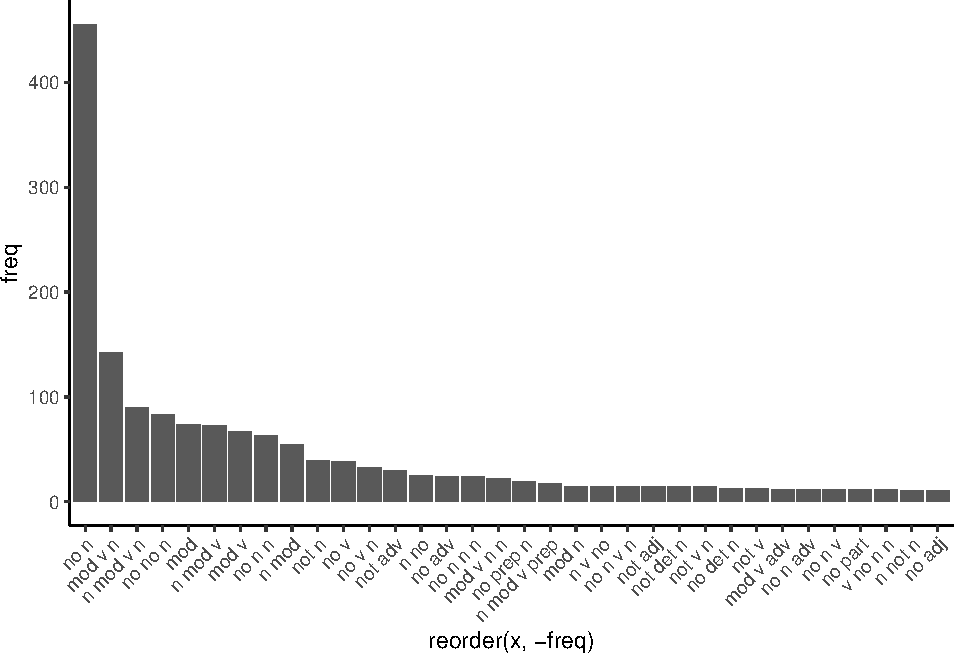
\includegraphics{negation_production_files/figure-latex/construction-1.pdf}
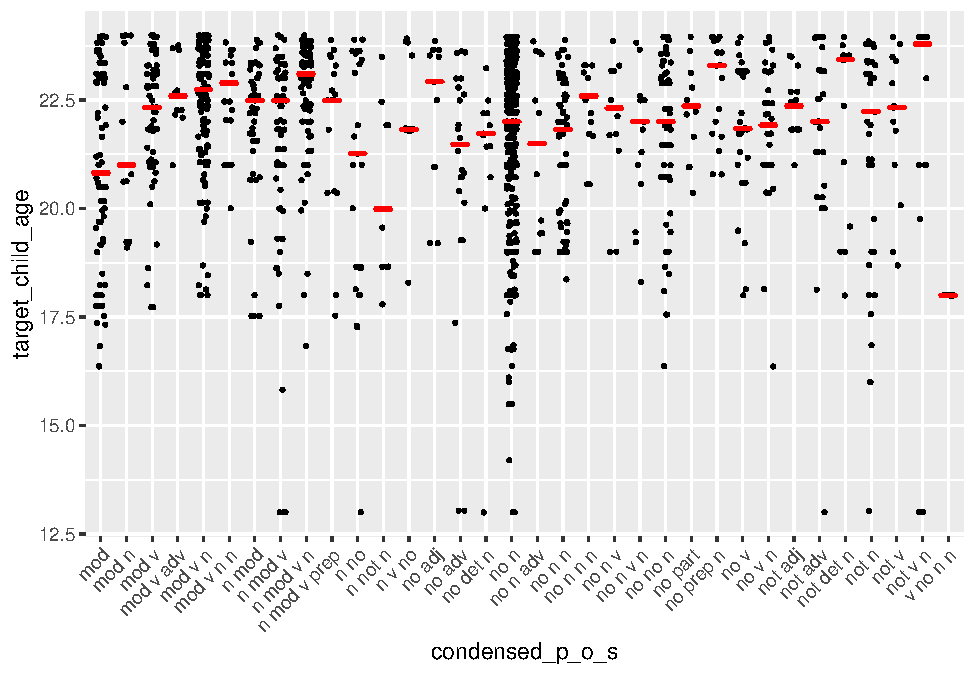
\includegraphics{negation_production_files/figure-latex/construction-2.pdf}

\begin{verbatim}
##   [1] no baby          no mama          no door          no car          
##   [5] no pillow        no straws        no game          no pages        
##   [9] no bath          no celery        no house         no milk         
##  [13] no box           no boot          no baseball      no caca swing   
##  [17] no supper        no cuppie        no thank_you     no car carpark  
##  [21] no color         no cat           no back          no water        
##  [25] no bubble        no juice         no milk          no nose         
##  [29] no way           no goggie        no letter        no pen          
##  [33] no puppy         no orange        no cookie        no glove        
##  [37] no horsie        no play          no pentagon      no moon         
##  [41] no boats         no book          no cars          no bricks       
##  [45] no park          no tickle        no toys          no touch        
##  [49] no man           no tape          no bite          no nana         
##  [53] no baby's        no bits          no egg           no machine      
##  [57] no mail          no tractor       no Ma            no tanker tanker
##  [61] no right         no lady          no bug           no wood         
##  [65] no babies        no pocket        no move          no push         
##  [69] no teddy         no walk          no bed           no dolls        
##  [73] no no monkeys    no couch         no mom           no shoe shoe    
##  [77] no mummy         no hold          no kisses        no blue         
##  [81] no no no powder  no powder        no clock         no valentines   
##  [85] no cream         no bottle        no train         no bus          
##  [89] no doll          no soup          no tigers        no pigs         
##  [93] no cheese        no girl          no window        no paper        
##  [97] no face          no mummy's       no boy           no mommy        
## [101] no pictures      no picture       no hands         no fall         
## [105] no soda          no lady          no food          no rice         
## [109] no truck         no bucket        no noise         no eggs         
## [113] no knee          no shoes         no socks         no baba         
## [117] no tea           no bee           no sir           no balloons     
## [121] no balloon       no motorcycle    no fork          no dance        
## [125] no work          no nappie        no glue          no cookies      
## [129] no works         no daddy's       no squirrel      no pink         
## [133] no cakes         no wheels        no yellow       
## 1807 Levels: a don't turn a ice no ice+cream a no ... Zoe not Zoe
\end{verbatim}

\begin{verbatim}
##  [1] no more stuff     no more people    no more people   
##  [4] no more ball      no no car         no no paint      
##  [7] no more bath      no more toy       no more juice    
## [10] no more machine   no more noise     no more light    
## [13] no more fire      no no mouse       no no pram       
## [16] no more pegs      no more car       no more apple    
## [19] no more blocks    no more monkey    no more squirrels
## [22] no more whale     no more wheels    no other pennys  
## [25] no more horse     no more meat     
## 1807 Levels: a don't turn a ice no ice+cream a no ... Zoe not Zoe
\end{verbatim}

\begin{verbatim}
##  [1] no push     no hat      no dada     no mommy    no fish    
##  [6] no pig      no bottle   no juice    no mommy    no picture 
## [11] no sweeties no uncle    no hug      no boat     no match   
## [16] no neck un  no pink     no monkey   no boy     
## 1807 Levels: a don't turn a ice no ice+cream a no ... Zoe not Zoe
\end{verbatim}

\begin{verbatim}
##  [1] no Mummy                  no Mommy                 
##  [3] no Mum                    no Baura                 
##  [5] no Joshua                 no Papa                  
##  [7] no Jen                    no Mom                   
##  [9] no Brittany               no Naima                 
## [11] no Nana                   no Fraser                
## [13] no Davy                   no Fraser no Fraser      
## [15] no Ma                     no No                    
## [17] no Mumm                   no Zita                  
## [19] no Daddy                  no Percy                 
## [21] no Toby                   no Nana's                
## [23] no Mummy's                no Abi                   
## [25] no Pooh                   no Mommy                 
## [27] no Papa                   no Eve                   
## [29] no Ernie                  no Pat                   
## [31] no Emily                  no Mama                  
## [33] no Laura_Lastname         no Mummy                 
## [35] no Carl                   no Thomas                
## [37] no Thomas_the_Tank_engine
## 1807 Levels: a don't turn a ice no ice+cream a no ... Zoe not Zoe
\end{verbatim}

\begin{verbatim}
##  [1] can't catch it      don't want it       can't do it        
##  [4] can't get it        don't touch it      don't do it        
##  [7] can't have it       tan't blow it       don't throw it     
## [10] don't like it       can't reach it      don't touch you    
## [13] didn't eat it       can't open it       don't hear you     
## [16] don't pour it       don't eat it        don't don't pour it
## [19] can't fix it        don't lose it       can't find it      
## [22] don't push it      
## 1807 Levels: a don't turn a ice no ice+cream a no ... Zoe not Zoe
\end{verbatim}

\begin{verbatim}
## [1] no more      no noone     no one       no more      no everybody
## 1807 Levels: a don't turn a ice no ice+cream a no ... Zoe not Zoe
\end{verbatim}

\begin{verbatim}
## [1] don't          can't can't    can't          can't         
## [5] don't          don't don't    doo+doos can't
## 1807 Levels: a don't turn a ice no ice+cream a no ... Zoe not Zoe
\end{verbatim}

\begin{verbatim}
## [1] I don't    I didn't   I can't    I couldn't I can't    I won't   
## [7] she don't  I won't   
## 1807 Levels: a don't turn a ice no ice+cream a no ... Zoe not Zoe
\end{verbatim}

\begin{verbatim}
##  [1] don't go           don't talk         can't catch       
##  [4] don't know         can't come         don't touch       
##  [7] don't kick         can't put          doesn't work      
## [10] don't fit          don't want         don't cry         
## [13] don't worry        leebs don't know   can't push        
## [16] don't jump         don't wiggle       can't reach       
## [19] don't push         can't move         don't nurse       
## [22] can't open         willn't fit        won't open        
## [25] willn't willn't go can't eat          don't put         
## [28] willn't work       don't throw        don't stop        
## [31] won't go           can't talk        
## 1807 Levels: a don't turn a ice no ice+cream a no ... Zoe not Zoe
\end{verbatim}

\begin{verbatim}
##  [1] don't touch that  don't do that     don't want that  
##  [4] don't want these  don't say that    didn't put this  
##  [7] didn't took this  don't put that    don't do this    
## [10] don't want this   don't spoil that  don't like that  
## 1807 Levels: a don't turn a ice no ice+cream a no ... Zoe not Zoe
\end{verbatim}

\begin{verbatim}
##  [1] I don't know           I don't play           I can't open          
##  [4] I don't remember       they don't fit         I can't tie           
##  [7] I don't come           I can't sing           hh I can't sing with  
## [10] my can't eat           I don't want           I didn't cry          
## [13] I couldn't predict     I can't go living+room I don't blanket       
## [16] I can't see           
## 1807 Levels: a don't turn a ice no ice+cream a no ... Zoe not Zoe
\end{verbatim}

\begin{verbatim}
##  [1] no read          no write         no pooped        no go           
##  [5] no want          no zipper        no want din+dins no draw         
##  [9] no bumble        no draw          no sit           no go bathroom  
## [13] no eat           no fit           no finish        no f finish     
## [17] no think         no left         
## 1807 Levels: a don't turn a ice no ice+cream a no ... Zoe not Zoe
\end{verbatim}

\begin{verbatim}
##  [1] I don't want it     I don't see it      I can't do it      
##  [4] I can't find it     I don't need it     I can't see you    
##  [7] I don't like it     I can't hear you    I didn't like it   
## [10] I can't see it      I can't can't do it
## 1807 Levels: a don't turn a ice no ice+cream a no ... Zoe not Zoe
\end{verbatim}

\begin{verbatim}
##  [1] not there     not again     not yet       not quite     not here     
##  [6] not off       not not there not on        not now       not asleep   
## 1807 Levels: a don't turn a ice no ice+cream a no ... Zoe not Zoe
\end{verbatim}

\begin{verbatim}
##  [1] no have black   no sit chair    no eat lunch    no have cracker
##  [5] no want truck   no want paint   no want food    no spill milk  
##  [9] no eat milk     no want bottle 
## 1807 Levels: a don't turn a ice no ice+cream a no ... Zoe not Zoe
\end{verbatim}

\begin{verbatim}
## # A tibble: 924 x 2
##    part_of_speech                        utterances                        
##    <fct>                                 <chr>                             
##  1 adj co                                hot no,wet no                     
##  2 adj cop pro:per                       naughty isn't it,cold isn't it    
##  3 adj mod v                             mum don't know                    
##  4 adj n co conj mod v                   little bun birthday ho but can't ~
##  5 adj n co n:prop coord n:prop coord n~ big kids like Emmy and Carl and L~
##  6 adj n neg pro:dem                     just crayon not these             
##  7 adj prep n:prop n cop pro:per         close to Rachel's feet wasn't it  
##  8 adv aux                               there aren't                      
##  9 adv cop                               there isn't ,there isn't          
## 10 adv cop qn n                          there is no moon                  
## # ... with 914 more rows
\end{verbatim}

\begin{verbatim}
## [1] 0.6919721
\end{verbatim}

Susan's Questions: Are you sure it is a quantifier or a marker of
non-existence? Check the difference between no+N and no-more+N how about
single \enquote{no}s?

To do: 1. cluster the most frequent categories 2. look at the age
distribution for the cluster (what about the distribution of age in
communicative function: nonexistence, nondesire, imperative)

\subsection{Participants}\label{participants}

\subsection{Material}\label{material}

\subsection{Procedure}\label{procedure}

\subsection{Data analysis}\label{data-analysis}

\section{Results}\label{results}

\section{Discussion}\label{discussion}

\newpage

\section{References}\label{references}

\begingroup
\setlength{\parindent}{-0.5in} \setlength{\leftskip}{0.5in}

\hypertarget{refs}{}

\endgroup


\end{document}
